\subsection{Graded and Request-Conditioned Support}
\label{sec:support-results}
\subsubsection{Development population and measurement scope}
We compare seven support configurations on ten seen development sources selected by the pilot's predeclared category ordering, with two seeds per source. SOFT25, SOFT50, and SOFT75 vary the protection floor; REQUEST\_SOFT25 (memory-fixed) uses request-conditioned correction with unchanged source memory. AUTO\_DETAIL, U25\_KV, and FlowEdit N26 provide matched references.

Metrics were computed from native PNG outputs at $512\times512$. NCC covers the whole image; the boundary-spanning region permits only zero shift. Preservation MAE covers eight sources with nonempty complements of the official edit mask. The lemon-addition and crayon-style cases have full-image edit masks and are excluded only from that metric. Edit-region MAE uses all ten sources. Both region errors measure source departure in their specified support.

\begin{table*}[t]
\centering\small
\caption{Completed support study on the same ten development sources, two seeds per source. NCC is whole-image correlation, distinct from earlier local-pattern NCC. Preservation MAE uses eight sources; edit-region MAE uses ten. Runtime describes the recorded runs. No ranking by semantic success is implied by column order.}
\label{tab:r82-results}
\begin{tabular}{lrrrrrr}
\toprule
Configuration & Global MAE & NCC $\uparrow$ & Preservation MAE $\downarrow$ & Edit MAE & NFE & Time (s)\\
\midrule
AUTO\_DETAIL & 0.1885 & 0.5900 & 0.1798 & 0.1787 & 91 & 43.90\\
U25\_KV & 0.1250 & 0.7635 & 0.1114 & 0.1380 & 91 & 43.38\\
SOFT25 & 0.1480 & 0.7269 & 0.1386 & 0.1501 & 91 & 53.25\\
SOFT50 & 0.1326 & 0.7648 & 0.1217 & 0.1404 & 91 & 43.63\\
SOFT75 & 0.1273 & 0.7668 & 0.1147 & 0.1384 & 91 & 43.71\\
\shortstack[l]{REQUEST\_SOFT25\\(memory-fixed)} & 0.1227 & 0.7446 & 0.1060 & 0.1464 & 97 & 45.42\\
FlowEdit N26 & 0.1271 & 0.7163 & 0.1032 & 0.1645 & 52 & 30.78\\
\bottomrule
\end{tabular}
\end{table*}

\subsubsection{Graded coverage restores global protection}
Increasing the support floor from 0.25 to 0.75 reduces preservation MAE from 0.139 to 0.115 and raises whole-image NCC from 0.727 to 0.767. SOFT75 approaches U25's preservation error of 0.111. The paired preservation-error difference SOFT75 minus U25 is $+0.00329$, with a source-bootstrap 95\% interval $[0.00211,0.00483]$. Its NCC difference is $+0.00324$ with interval $[-0.00031,0.00687]$. These results explain the recovery through broader correction coverage: the high-floor configuration behaves close to the global endpoint.

\subsubsection{Request-conditioned support and matched references}
REQUEST\_SOFT25 uses Eq.~\eqref{eq:request-support}, with native source and target evaluations at three common reference states. The response map is fixed before generation and uses no official evaluation region. Memory still acts on all image queries in the first seven steps.

REQUEST\_SOFT25 has preservation MAE 0.10601, with a paired difference from U25 of $-0.00543$ and interval $[-0.01180,0.00072]$. Against quarter-floor contrast support SOFT25, preservation MAE decreases from 0.13863 by 23.5\%; all eight eligible sources improve after seed averaging. That paired difference is $-0.03262$, with exploratory 95\% interval $[-0.04727,-0.02020]$. The global reference and contrast control distinguish the candidate's measured retention from the particular support it replaces.

\begin{table}[t]
\centering\footnotesize
\caption{Source-paired effects on preservation MAE. Difference is first method minus second; negative values favor the first. Each source contributes the mean of its two seeds. Intervals use 10,000 source-bootstrap resamples without multiple-comparison adjustment. REQUEST abbreviates REQUEST\_SOFT25 (memory-fixed).}
\label{tab:r82-paired}
\begin{tabular}{lrr}
\toprule
Comparison & Difference & 95\% interval\\
\midrule
REQUEST $-$ SOFT25 & $-0.03262$ & $[-0.04727,-0.02020]$\\
REQUEST $-$ U25 & $-0.00543$ & $[-0.01180,0.00072]$\\
SOFT50 $-$ U25 & $0.01026$ & $[0.00734,0.01415]$\\
SOFT75 $-$ U25 & $0.00329$ & $[0.00211,0.00483]$\\
\bottomrule
\end{tabular}
\end{table}

\subsubsection{Magnitude and computation}
All four new arms use the same ONLINE coefficient $a=0.25$, evaluated on each arm's own evolving state. Their mean cumulative correction impulses are 0.24172 (SOFT25), 0.23501 (SOFT50), 0.23296 (SOFT75), and 0.23063 for REQUEST\_SOFT25 (memory-fixed), compared with 0.23191 for U25. Thus this experiment compares a shared normalization rule; trajectories determine the realized cross-arm doses. The request estimator adds six transformer calls, giving 97 standalone NFE versus 91 for graded support, an increase of 6.6\%. Its recorded runtime is 45.42 seconds. Run-level timing variability is documented in the provenance appendix.

\subsubsection{Requested edits and visible failure categories}
All twenty comparison sheets were inspected against the source and target prompts. Figure~\ref{fig:r82-qualitative} shows a relational failure, a seed-specific successful addition, and a style/geometry case. The examples distinguish object presence, requested relations, and rendering artifacts.

\begin{figure*}[t]
\centering
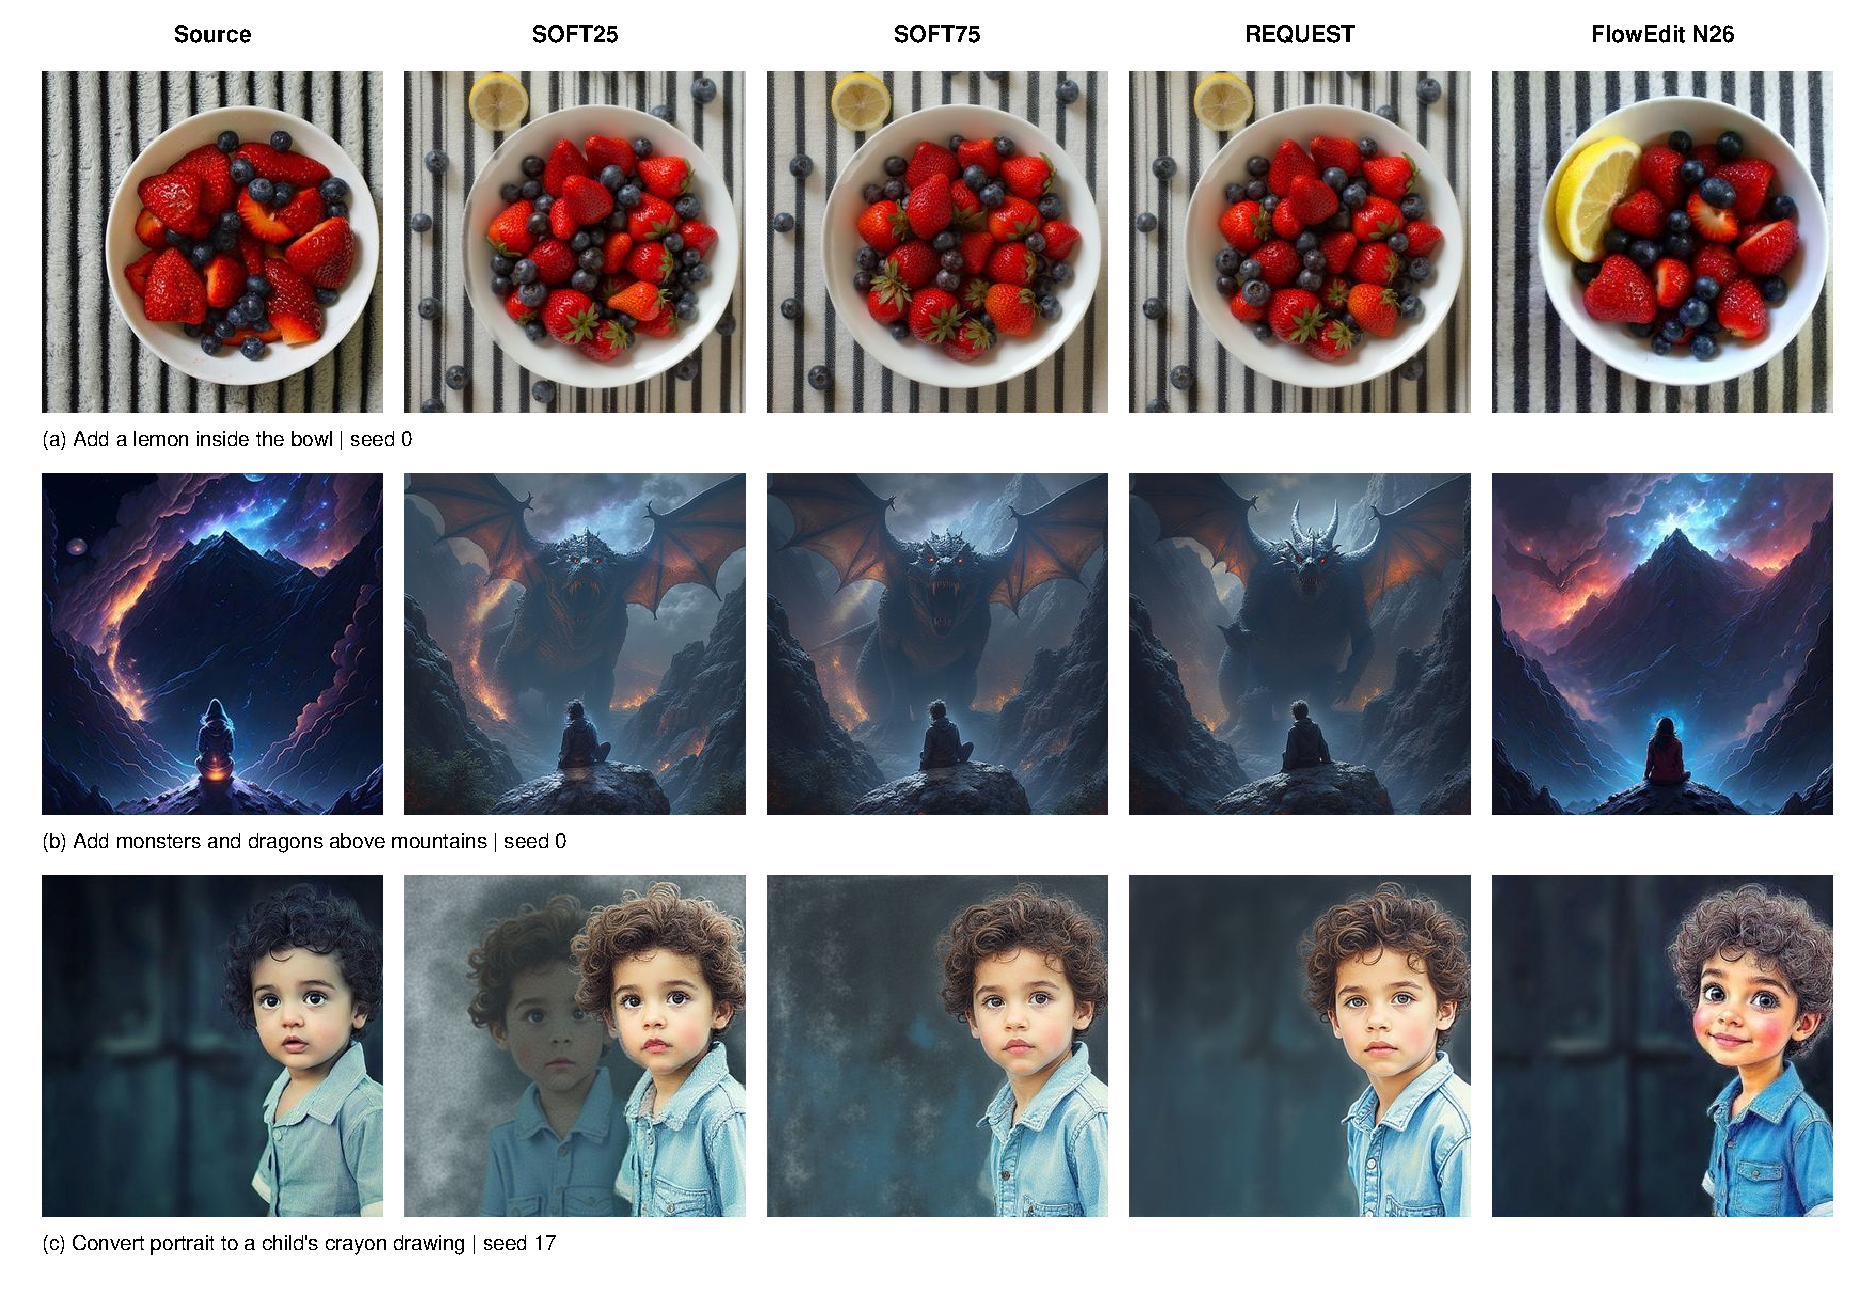
\includegraphics[width=.98\textwidth]{figures/r82_request_examples.pdf}
\caption{Selected completed support-study outputs. Rows show: adding a lemon inside the berry bowl (seed 0), adding monsters and dragons above mountains (seed 0), and converting a portrait to a child's crayon drawing (seed 17). REQUEST\_SOFT25 (memory-fixed) places the lemon beside the bowl; FlowEdit places it inside in this seed. The request/soft variants generate a visible dragon in the second row. In the third row REQUEST\_SOFT25 (memory-fixed) reduces the prominent duplicate-face structure visible in SOFT25, while the requested crayon appearance remains weak. Examples illustrate distinct outcomes, not aggregate success rates.}
\label{fig:r82-qualitative}
\end{figure*}

Across both seeds, the pepper-under-towel request leaves the pepper on top. Lemon addition often produces the requested object outside the bowl. Yellow-kitten outputs vary between partial cream coloration and stronger orange coloration with changed pose. Rough-sea edits often produce waves, with an extra foreground structure in one REQUEST\_SOFT25 (memory-fixed) output. Glass-to-wood and crystal-lamp requests produce changes in opacity or decoration with inconsistent target material. Olive removal often succeeds alongside changes to bowls, cloth, or surrounding objects. Wolf and dragon requests show visible semantic changes in some outputs. The portrait-style task retains rendered portrait appearance in many outputs, with varying duplicate-face artifacts. These findings motivate measuring requested relations and attributes alongside retention.
